\documentclass[11pt,reqno]{amsart}
\usepackage[top=1in, left=1in, right=1in, bottom=1in]{geometry}                % See geometry.pdf to learn the layout options. There are lots.
\geometry{letterpaper}                   % ... or a4paper or a5paper or ...
\usepackage[parfill]{parskip}    % Activate to begin paragraphs with an empty line rather than an indent
%\usepackage{algorithm, algorithmic}

\usepackage{algorithm}
\usepackage{algpseudocode}

\usepackage{graphicx}

\usepackage{verbatim}
\usepackage{amssymb}
\usepackage{amsmath}

\usepackage{enumitem}

\usepackage{setspace}
\doublespacing

\usepackage{natbib}

%\usepackage{epstopdf}
%\DeclareGraphicsRule{.tif}{png}{.png}{`convert #1 `dirname #1`/`basename #1 .tif`.png}

\newcommand{\RR}{I\!\!R} %real numbers
\DeclareMathOperator{\diag}{diag}

\algnewcommand{\Inputs}[1]{%
  \State \textbf{Inputs:}
  \Statex \hspace*{\algorithmicindent}\parbox[t]{.8\linewidth}{\raggedright #1}
}
\algnewcommand{\Initialize}[1]{%
  \State \textbf{Initialize:}
  \Statex \hspace*{\algorithmicindent}\parbox[t]{.8\linewidth}{\raggedright #1}
}

\title[RVD3]{Variant detection model with improved robustness and accuracy for low-depth targeted next-generation sequencing data}
\author{}
%\date{}                                           % Activate to display a given date or no date

\begin{document}

\begin{abstract}

We analyzed the Sensitivity of the Bayesian model to different priors. Jeffreys prior improves robustness and accuracy of Single Nucleotide Variant detection algorithm.

\end{abstract}

\maketitle

%%%%%%%%%%%%%%%%%%
% Introduction
%%%%%%%%%%%%%%%%%%
\section{Introduction}

Massively parallel sequencing data were generated by Next-generation sequencing (NGS) technology to benefit clinical diagnostics and sequencing based phylogenetic analyses. One primary application of NGS is variation detection among related populations and separate novel single-nucleotide variants(SNV) candidates.
Currently SNV are deduced on NGS platform by variants calling algorithms. Typically, SAMtools[XX], Genome Analysis Toolkit (GATK) [XX], VarScan2[XX], and SPLINTER[XX] are all highly used in detecting low-frequency variants. However identifying true SNVs remains challenging because of high false positive rates or high false discovery rate. Another statistical method-RVD, was proposed based on beta-binomial model for ultrasensitive rare single nucleotide variant detection. So based on the RVD hierarchical model we built an improved robustness and accuracy model for low-depth variants detection.


%%%%%%%%%%%%%%%%%%
% Data Sets
%%%%%%%%%%%%%%%%%%
\section{Data Sets}

\subsection{Synthetic DNA Sequence Data}

Two 400bp DNA sequences differ only 14 single nucleotide positions. Sample of the case and control DNA were mixed to yield 0.1\%, 0.3\%, 1\%, 10\%, and 100\% defined minor allele frequencies (MAFs). The details of the experimental protocol are available from the original publication~\citep{Flaherty:2011ja}. We used BWA v0.7.5a to align the reads to the reference sequence with the -C50 option to remove the reads of high mapping quality. BAM files were sampled by $10\times$, $100\times$, $1,000\times$, and $10,000\times$ using Picard v1.104. The final data set contains read pairs for $N=6$ replicates for the control at different MAF levels.

\subsection{Yeast Data}
We first mapped the GSY1135 to Chromosome 10 in S288c reference genome by BWA v0.7.5a [XXX]. Then called SNPs by GATK UnifiedGenotyper and created a FASTA GSY1135 reference using GATK FastaAlternative [XXX].
Secondly, we downloaded generation 7 as control and generation 133 as case in experiment 1 from [XXX], and removed WT population using FASTX Barcode Splitter [XXX] and trimed the Nextera tag by Cutadapt v1.3.
Finally, the FASTQ files of case and control were mapped to GSY1135 reference and pileup files were generated using Samtools v0.1.19.

%%%%%%%%%%%%%%%%%%
% RVD3 Model
%%%%%%%%%%%%%%%%%%
\section{RVD3 Model}

\subsection{Model Structure}\label{sec:model_structure}
RVD3 is based on a hierarchical Bayesian model. Through hypothesis test on case and control samples by RVD3, we can call the variants sucsessfully. Now the definitions for sample data are given: $r_{ji}$ is the number of reads with a non-reference base at position $j$ in replicate $i$, and $n_{ji}$ is the total number of reads at position $j$ in replicate $i$. Three parameters of the model are: $\mu_0$, a global error rate; $M_0$, the global position which estimates the variation in the error rate across the positions; priors for $M_j$, two kinds of priors are log-normal prior and Jeffreys prior, which enhanced the former RVD model [XXX]. Here $M_j$ is the local precision measures the alteration in the error rate across replicates at position $j$. The graphical chart for RVD3 are shown in Figure~\ref{fig:graphical_model}.
RVD3 hierarchically includes four levels of samplings: $r_{ji} | n_{ji} \thicksim \text{Binomial}(\theta_{ji}, n_{ji})$ models the variation due to sampling the pool of DNA molecules on the sequencer. $\theta_{ji} \thicksim \text{Beta}(\mu_j, M_j)$ models the variation caused by experimental repeatability. The variation in error rate due to sequence context is modeled by $\mu_j \thicksim \text{Beta}(\mu_0, M_0)$. And the local precision is modeled by $ M_{j} \thicksim \text{log-normal}(\mu, \sigma)$ (log-normal prior), and $\pi\left({M}_{j}\right)$ (Jeffreys prior).

\begin{figure}[h]
\begin{center}
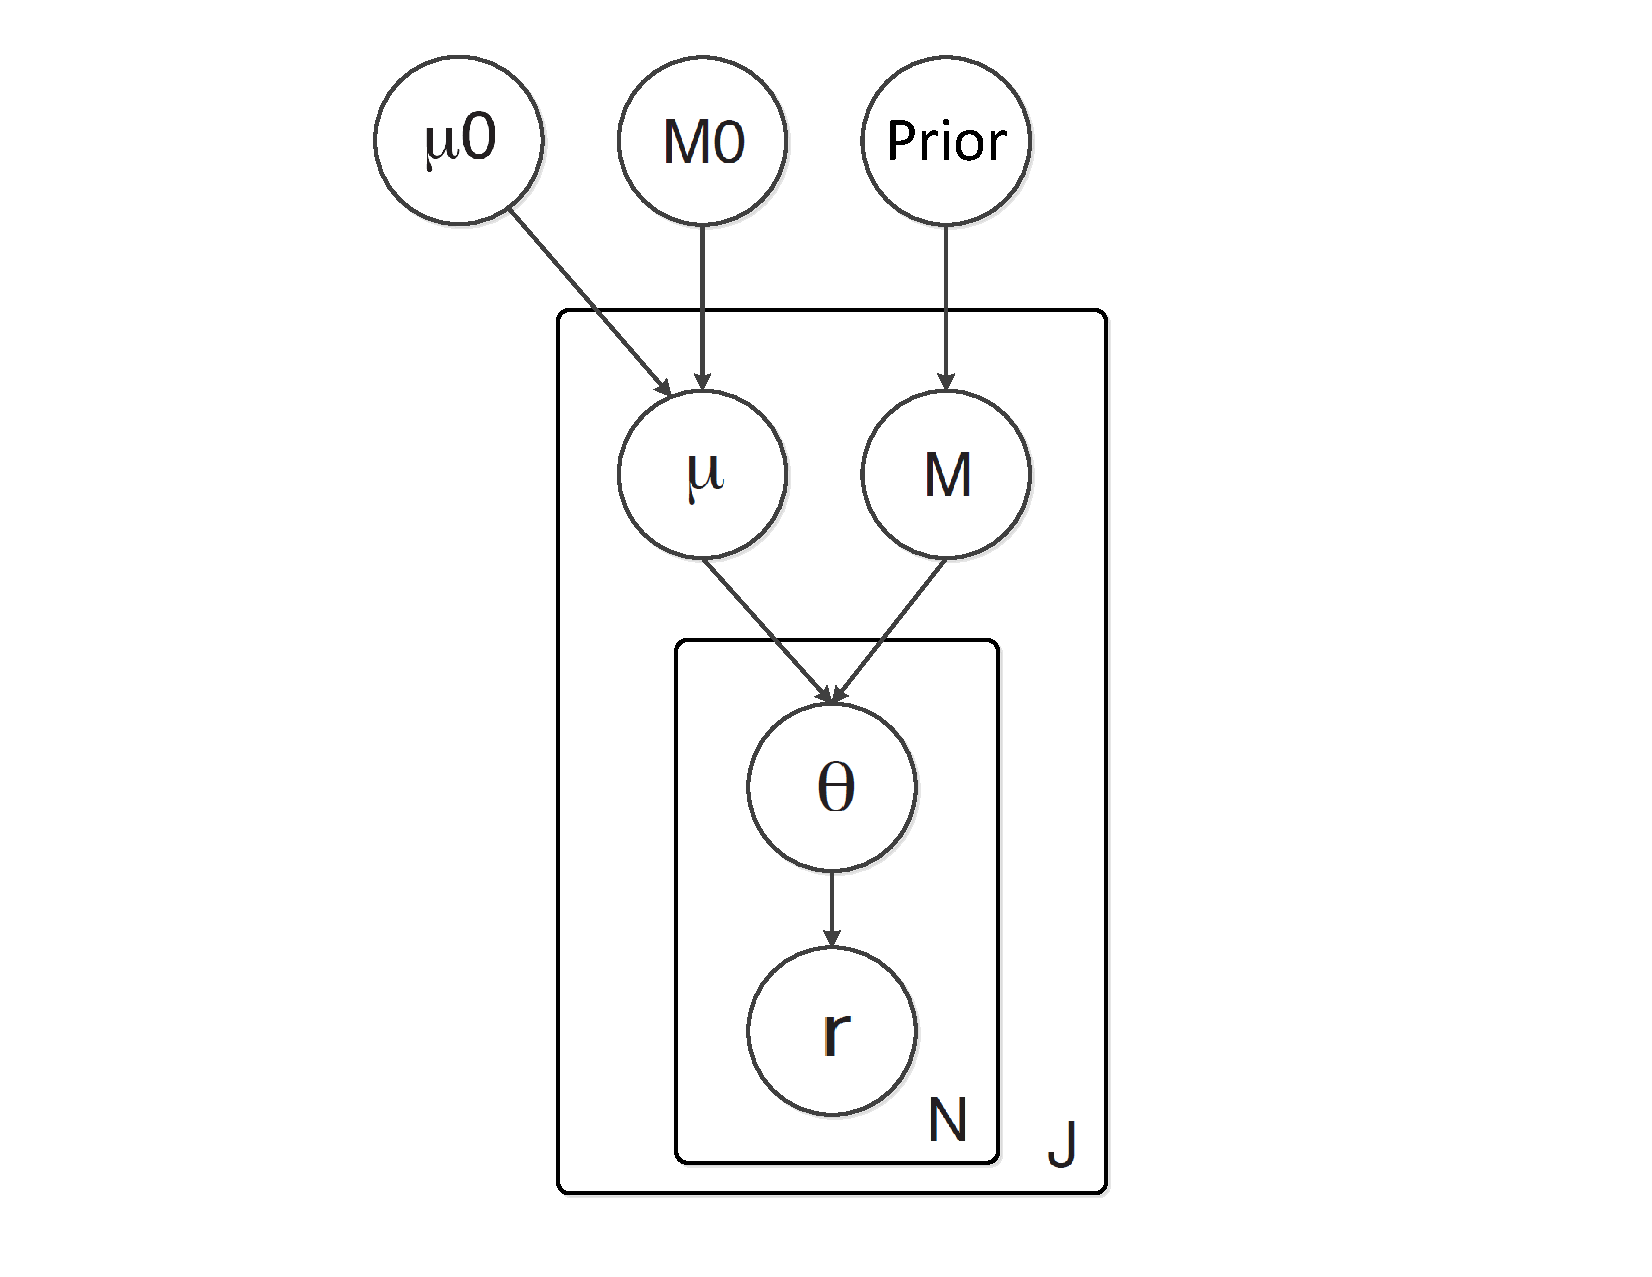
\includegraphics[width=100mm]{figs/RVD3_model.pdf}
\caption{RVD3 Graphical Model}
\label{fig:graphical_model}
\end{center}
\end{figure}


%%%%%%%%%%%%%%%%%%
% Inference & Hypothesis Testing
%%%%%%%%%%%%%%%%%%
\subsection{Inference and Hypothesis Testing}

\begin{algorithm}[ht]
\caption{Inference process for Metropolis-within-Gibbs}
\label{alg:metro_gibbs}
\begin{algorithmic}[1]

\State Initialize $\theta$, $\mu$, $M_j$, $\mu_0$, $M_0$
\Repeat
\For {each location j}
  \State Draw T samples from $p \left( \mu_j |\theta_{ij},\mu_0,M_0\right)$ using M--H \Comment{Sample $\mu_j$}
  \State Set $\mu_j$ to the sample median for the T samples
  \State Draw T samples from $p \left( M_{j} |\mu,\sigma, \theta_{ji},\mu_j\right)$ using M--H \Comment{Sample $M_j$}

  \For {each replicate i}
	\State Sample from $p \left( \theta_{ij} |r_{ij},n_{ij},\mu_j,M \right)$  \Comment{Sample $\theta_{ji}$}
  \EndFor

\EndFor
\Until {sample size sufficient}
\end{algorithmic}
\end{algorithm}

Metropolis-within-Gibbs sampling is evolved for inference. Algorithm 1 shows the inference process and the detail are also illustrated.

%%%%%%%%%%%%%
% Initialization
%%%%%%%%%%%%%
\subsubsection{Initialization}
The initial values for the model parameters and latent variables is obtained by a method-of-moments (MoM) procedure. MoM works by setting the population moment equal to the sample moment. A system of equations is formed such that the number of moment equations is equal to the number of unknown parameters and the equations are solved simultaneously to give the parameter estimates. We simply start with the data matrices $r$ and $n$ and work up the hierarchy of the graphical model solving for the parameters of each conditional distribution in turn.

We present the initial parameter estimates here and provide the derivations in Appendix~\ref{sec:appendix_mom}. The MoM estimate for replicate-level parameters are
$\tilde{\theta}_{ji} = \frac{r_{ji}} {n_{ji}}$.
The estimates for the position-level parameters are
$\tilde{\mu}_j = \frac{1}{N} \sum_{i=1}^N \theta_{ji}$
and
$\tilde{M_j} = \frac{ \tilde{\mu}_j (1 - \tilde{\mu}_j ) } { \frac{1}{N} \sum_{i=1}^N \theta_{ji}^2 } -1$.
The estimates for the genome-level parameters are
$\tilde{\mu}_0 = \frac{1}{J} \sum_{j=1}^J \mu_j$
and
$\tilde{M}_0 = \frac{ \tilde{\mu}_0 (1 - \tilde{\mu}_0 ) } {\frac{1}{J} \sum_{j=1}^J \mu_j^2 } -1$.
While MoM is known to have the potential to return estimates outside the true parameter bounds, we have not encountered such behavior in this application.

%%%%%%%%%%%%%%%%%%
% Sampling theta
%%%%%%%%%%%%%%%%%%
\subsubsection{Sampling from $p \left( \theta_{ij} |r_{ij},n_{ij},\mu_j,M \right)$}

Samples from the posterior distribution
$p(\theta_{ji} | r_{ji}, n_{ji}, \mu_j, M_j)$
are drawn analytically because of the Bayesian conjugacy between the prior
$p(\theta_{ji} | \mu_j, M_j) \thicksim \text{Beta}(\mu_j, M_j)$
and the likelihood
$p(r_{ji} | n_{ji}, \theta_{ji}) \thicksim \text{Binomial}(\theta_{ji}, n_{ji})$.
The posterior distribution is
\begin{equation}
	p(\theta_{ji} | r_{ji}, n_{ji}, \mu_j, M_j) \thicksim \text{Beta}\left( \frac{r_{ji} + M_j \mu_j}{n_{ji} + M_j} , n_{ji} + M_j\right).
\end{equation}

%%%%%%%%%%%%%%%%%%
% Sampling mu
%%%%%%%%%%%%%%%%%%
\subsubsection{Sampling from $p \left( \mu_j |\theta_{ji},M_j,\mu_0,M_0\right)$}
The posterior distribution over $\mu_j$ given its Markov blanket is
\begin{equation}
	p( \mu_j | \theta_{ji}, M_j, \mu_0, M_0 ) \propto p(\mu_j | \mu_0, M_0) p(\theta_{ji} | \mu_j, M_j).
\end{equation}

Since the prior, $p(\mu_j | \mu_0, M_0)$, is not conjugate to the likelihood, $p(\theta_{ji} | \mu_j, M_j)$, we cannot write an analytical form for the posterior distribution. Instead, we sample from the posterior distribution using the Metropolis-Hastings algorithm.

We fixed the proposal distribution variance for all the Metropolis-Hastings steps within a Gibbs iteration to $\sigma_j = 0.1 \cdot \mu_j^{(p)}$ if $\mu_j^{(p)} \in (10^{-3},1-10^{-3})$; otherwise, we set $\sigma_j = 10^{-4}$ if $\mu_j^{(p)}< 10^{-3}$ and $\sigma_j = 10^{-1}-10^{-4}$ if $\mu_j^{(p)}>1-10^{-3}$. Though it is not theoretically necessary, we have found that the algorithm performance improves when we take the median of five or more M-H samples as a single Gibbs step for each position.


We resampled from the proposal if the sample is outside of the support of the posterior distribution. We typically discard 20\% of the sample for burn-in and thin the chain by a factor of 2 to reduce autocorrelation among samples. Since, each position $j$ is exchangeable given the global hyperparameters $\mu_0$ and $M_0$ this sampling step can be distributed across up to $J$ processors.

%%%%%%%%%%%%%%%%%%
% Sampling Mj
%%%%%%%%%%%%%%%%%%
\subsubsection{Sampling from $p \left( M_{j} |\mu,\sigma, \theta_{ji},\mu_j\right)$}
For Jeffreys prior is from the Fisher information and ${\theta }_{ji}\sim Beta\left( {\mu }_{j},{M}_{j}\right)$,

\begin{equation}\label{equ:JefferyInference}
I\left({M}_{j}\right)={E}_{{M}_{j}}\left[ -\frac{\delta ^{2}\log p\left(\theta _{j}|\mu_{j},M_{j}\right)}{\delta M^{2}_{j}}\right]
\end{equation}

We calculated the equations (Appendix B) and obtained the Jeffreys' prior for $M_j$:

% \pi\left({M}_{j}\right) =
\begin{equation}
[-\left(\Psi_{1}(M_{j}) - \Psi_{1}(\mu_{j} M_{j})\mu_{j}^{2} - \Psi_{1}((1-\mu_{j})M_{j}){(1-\mu_{j})^{2}}\right)]^{\frac{1}{2}}
\end{equation}

For log-normal prior, the posterior distribution over $M_{j}$ given its Markov blanket is

\begin{equation}
	p( M_{j} |\mu, \sigma, \theta_{ji},\mu_j) \propto p(\theta_{ji} | \mu_j, M_j) p(M_{j} | \mu, \sigma)
\end{equation}

We have $ \theta_{ji}\thicksim\text{Beta}(\mu_{j},M_{j})$, and $ M_{j} \thicksim \text{log-normal}(\mu, \sigma)$. Since we cannot provide an intepretive form for it, so Metropolis-Hastings algorithm was used to sample from the posterior distribution.


%%%%%%%%%%%%%%%%%%
% Posterior Density Test
%%%%%%%%%%%%%%%%%%
\subsubsection{Posterior Density Test}\label{sec:hypothesis_test}
Posterior distributions of $\mu_j$ for the control and case are achieved-  $\tilde{\mu}_j^{\text{case}}$ and $\tilde{\mu}_j^{\text{control}}$, by Metropolis-within-Gibbs. So we called a variant when $\tilde{\mu}_j^{\text{case}} > \tilde{\mu}_j^{\text{control}}$ with $1-\alpha$ confidence,
\begin{equation}\label{eqn:bayes_test}
	\Pr( \tilde{\mu}_j^{\text{case}} - \tilde{\mu}_j^{\text{control}} \geq \tau ) > 1-\alpha,
\end{equation}
where $\tau$ is a detection threshold and $1-\alpha$ is the confidence level. We set $\tau = 0$ in our experiment [XXX].

%%%%%%%%%%%%%%%%%%
% Chi^2 Test
%%%%%%%%%%%%%%%%%%
% Limited in the 9 pages, so maybe considering neglect the Chi^2 Test since we show the results without Chi^2 Test.

%%%%%%%%%%%%%%%%%%%%%%%%
% Priors for precision parameter
%%%%%%%%%%%%%%%%%%%%%%%%
\subsection{Priors for precision parameter}
%\subsubsection{Improper Prior}
Playing no prior on $ M_{j}$ is an implicit improper prior. An improper prior integrates to infinity, and may cause an improper posterior which results in an invalid inferences [XXX]. Because an improper prior is a bad choice since a step has to be taken to confirm the posterior is proper. We considered about two typical priors: non-information prior - Jeffreys prior, and information prior - log-normal prior.

%\subsubsection{Jeffreys Prior}
Jeffreys prior is proposed to establish a least informative prior that is automatically invariant to transformations by Harold Jeffreys (1946). It is defined in terms of the Fisher information and works well with a single parameter. In our research Jeffreys prior for $M_j$ is the square root of Fisher information of $M_j$. Log-normal prior is a typical prior for the beta density's parameters, $\theta_{ji} \thicksim \text{Beta}(\mu_j, M_j)$. So log-normal prior was incorporated in the model. The parameters of it denoted $\mu$ (mean) and $\sigma$ (standard deviation) respectively.

%%%%%%%%%%%%%%%%%%
% Results
%%%%%%%%%%%%%%%%%%
\section{Results}

%%%%%%%%%%%%%%%%%%
% Sensitivity analysis of priors
%%%%%%%%%%%%%%%%%%
\subsection{Sensitivity analysis of priors}
In order to examine the robustness of RVD3 to changes of different priors, we performed information prior (log-normal) and non-information prior (Jeffreys). We found that RVD3 is robust to changing the priors. The RVD3 algorithm provides estimates of model parameters and latent variables given the data.

We show several of these parameters of the model with Jeffreys prior in Figure~\ref{fig:M_jeffrey}. The left column of is shows the read depth for each of the six BAM files (three replicates each with two read pairs) for each data set. Because the DNA was not sheared and ligated prior to sequencing, the read depth drops to zero at the boundaries. For the 100\% mutant data set, the read depth drops at the mutant locations. This is due to the parameters imposed at the alignment stage. The right column of Figure~\ref{fig:M_jeffrey} reveals the parameter estimates $\hat{M}_j$ and $\hat{M}_0$ for each data set. $M_j$ measures the variance between replicates at location $j$. There is little variability across positions indicating that the replication variance does not change greatly across position. Furthermore, $M_j$ from Jeffreys prior [Figure~\ref{fig:M_jeffrey}] across the M value drops at the mutant positions when the data is 10\% and 100\% mutant, which is not shown in log-normal prior [Figure~\ref{fig:M_lognormal}] in Appendix C. Additionally, the error rate across positions is captured by the $M_0$ parameter shown as a horizontal dotted line in the plots in the right column. $M_j$ is greater than $M_0$ the precision between replicates is higher than the precision across positions.

\begin{figure}[htbp]
\begin{center}
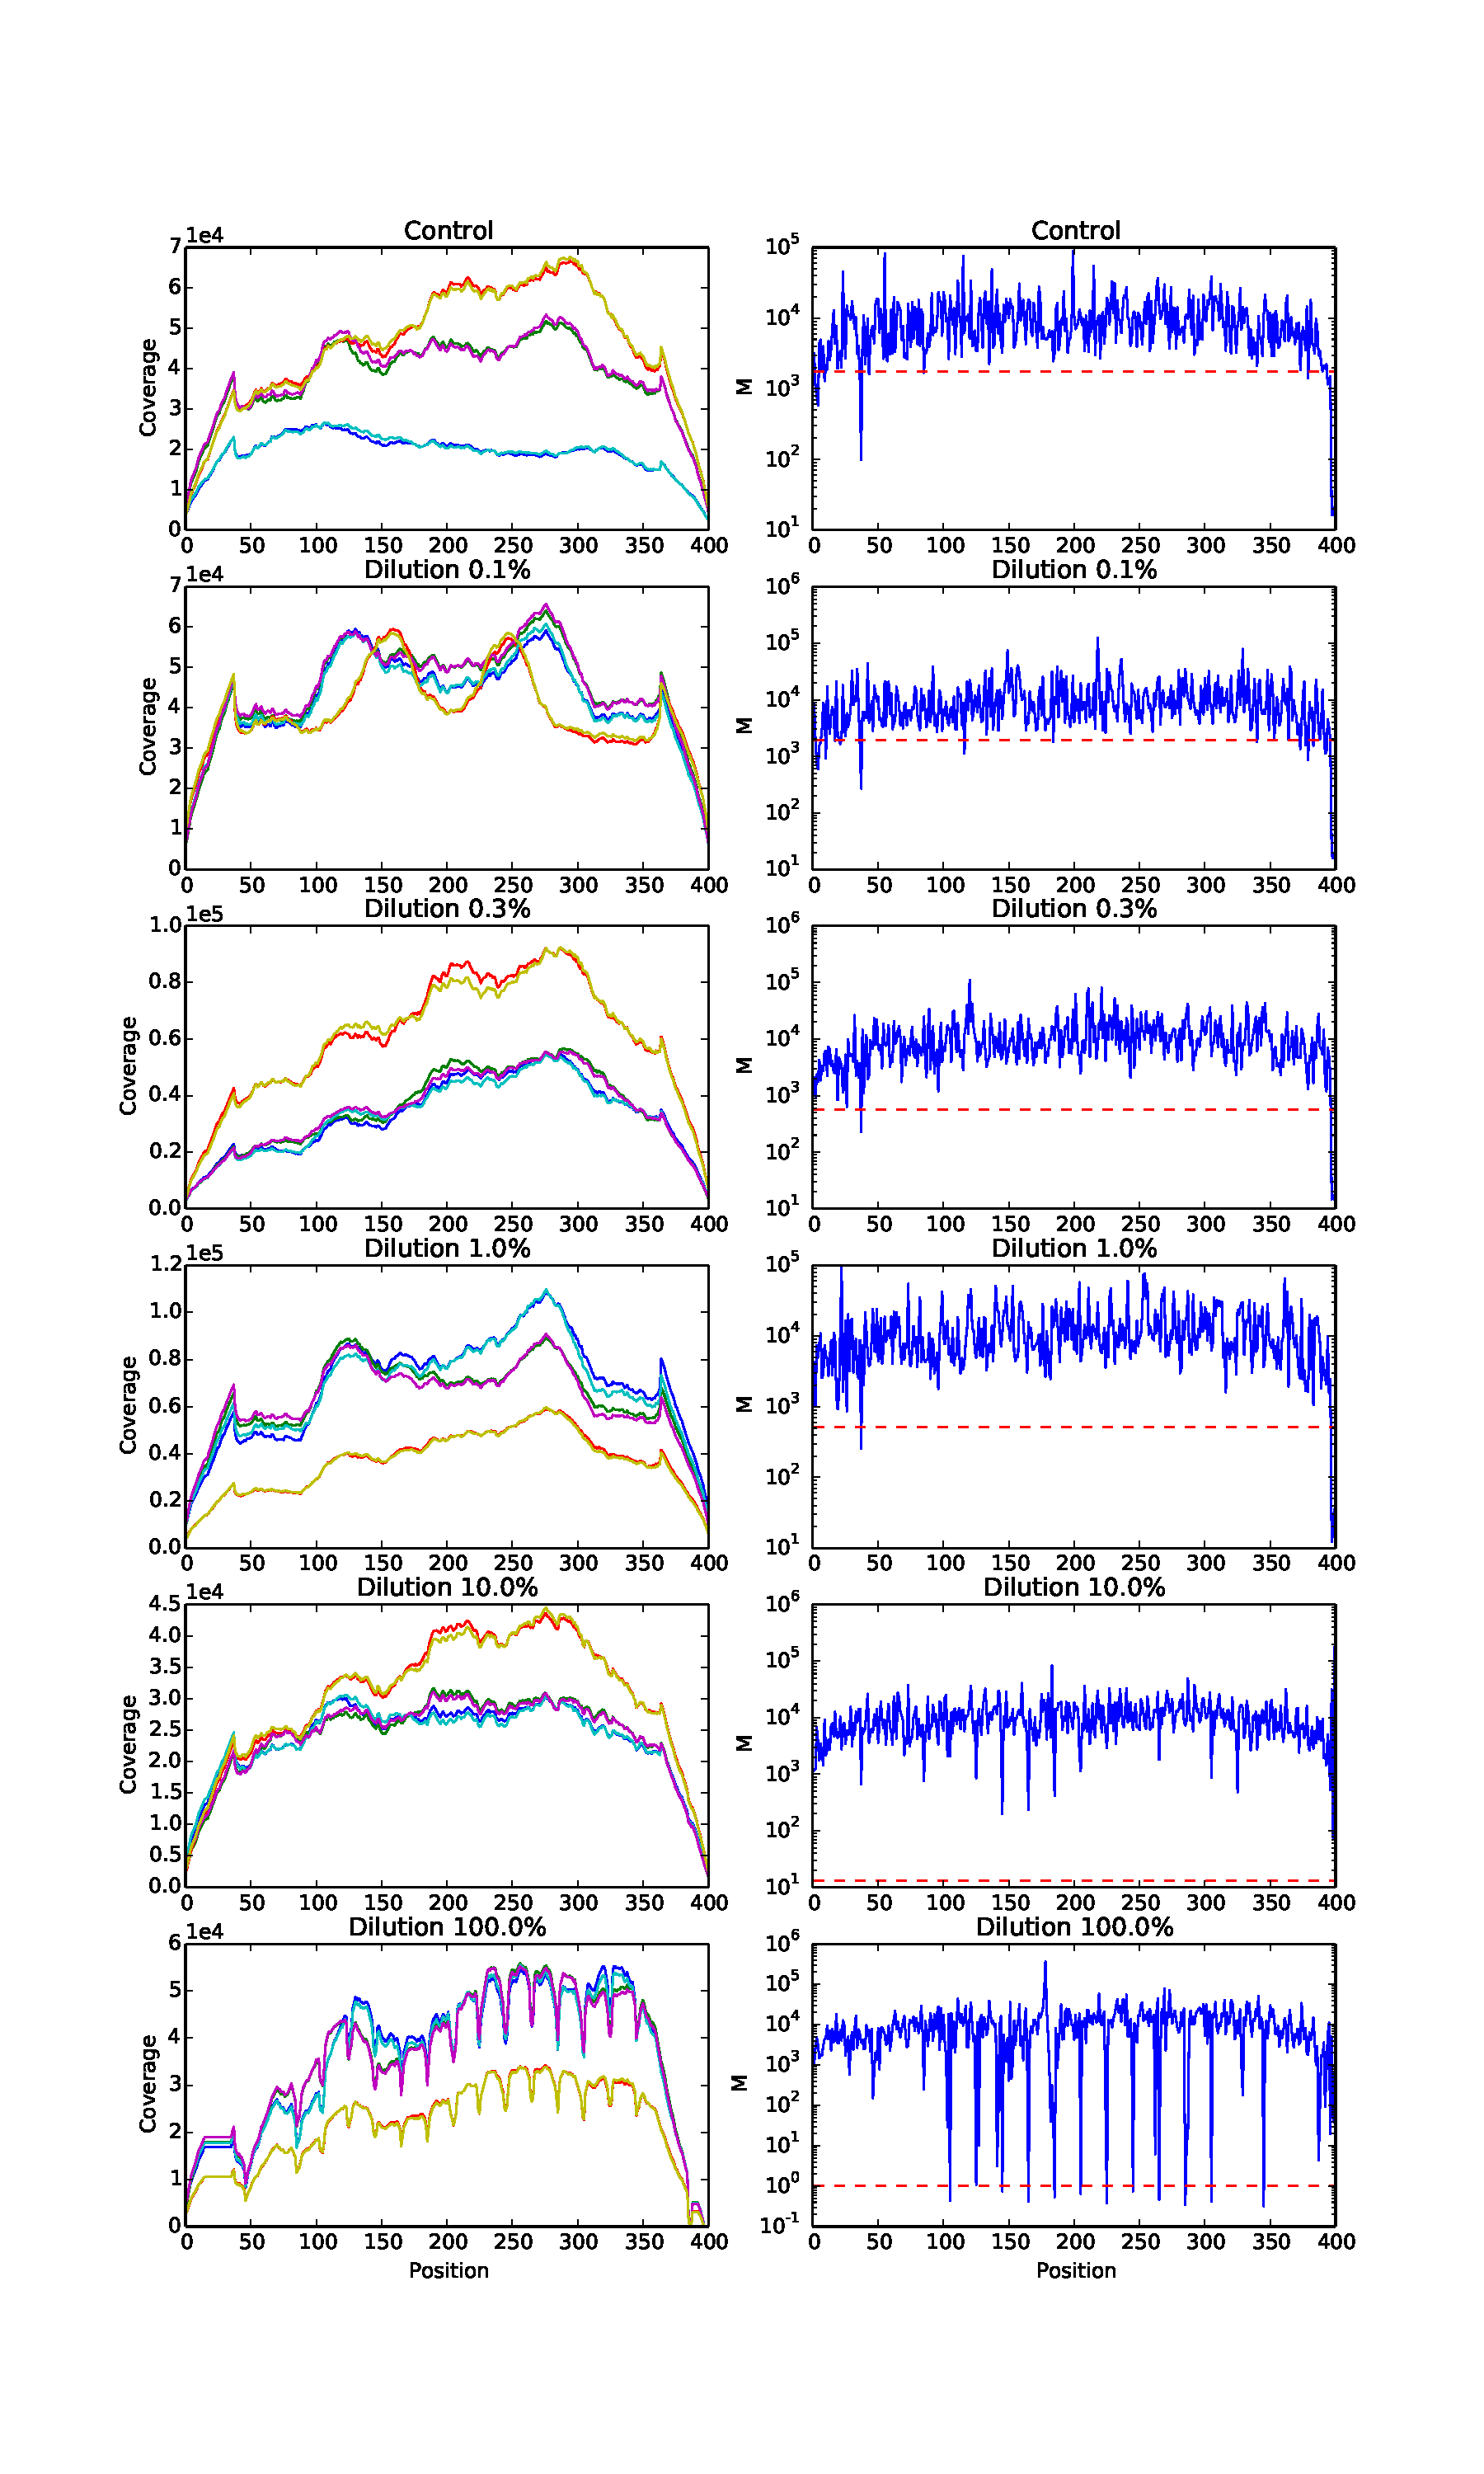
\includegraphics[width=120mm]{figs/M_jeffrey.pdf}
\caption{Key parameters for RVD3 model with Jeffreys prior for synthetic DNA data sets.}
\label{fig:M_jeffrey}
\end{center}
\end{figure}

\begin{figure}[htbp]
\begin{center}
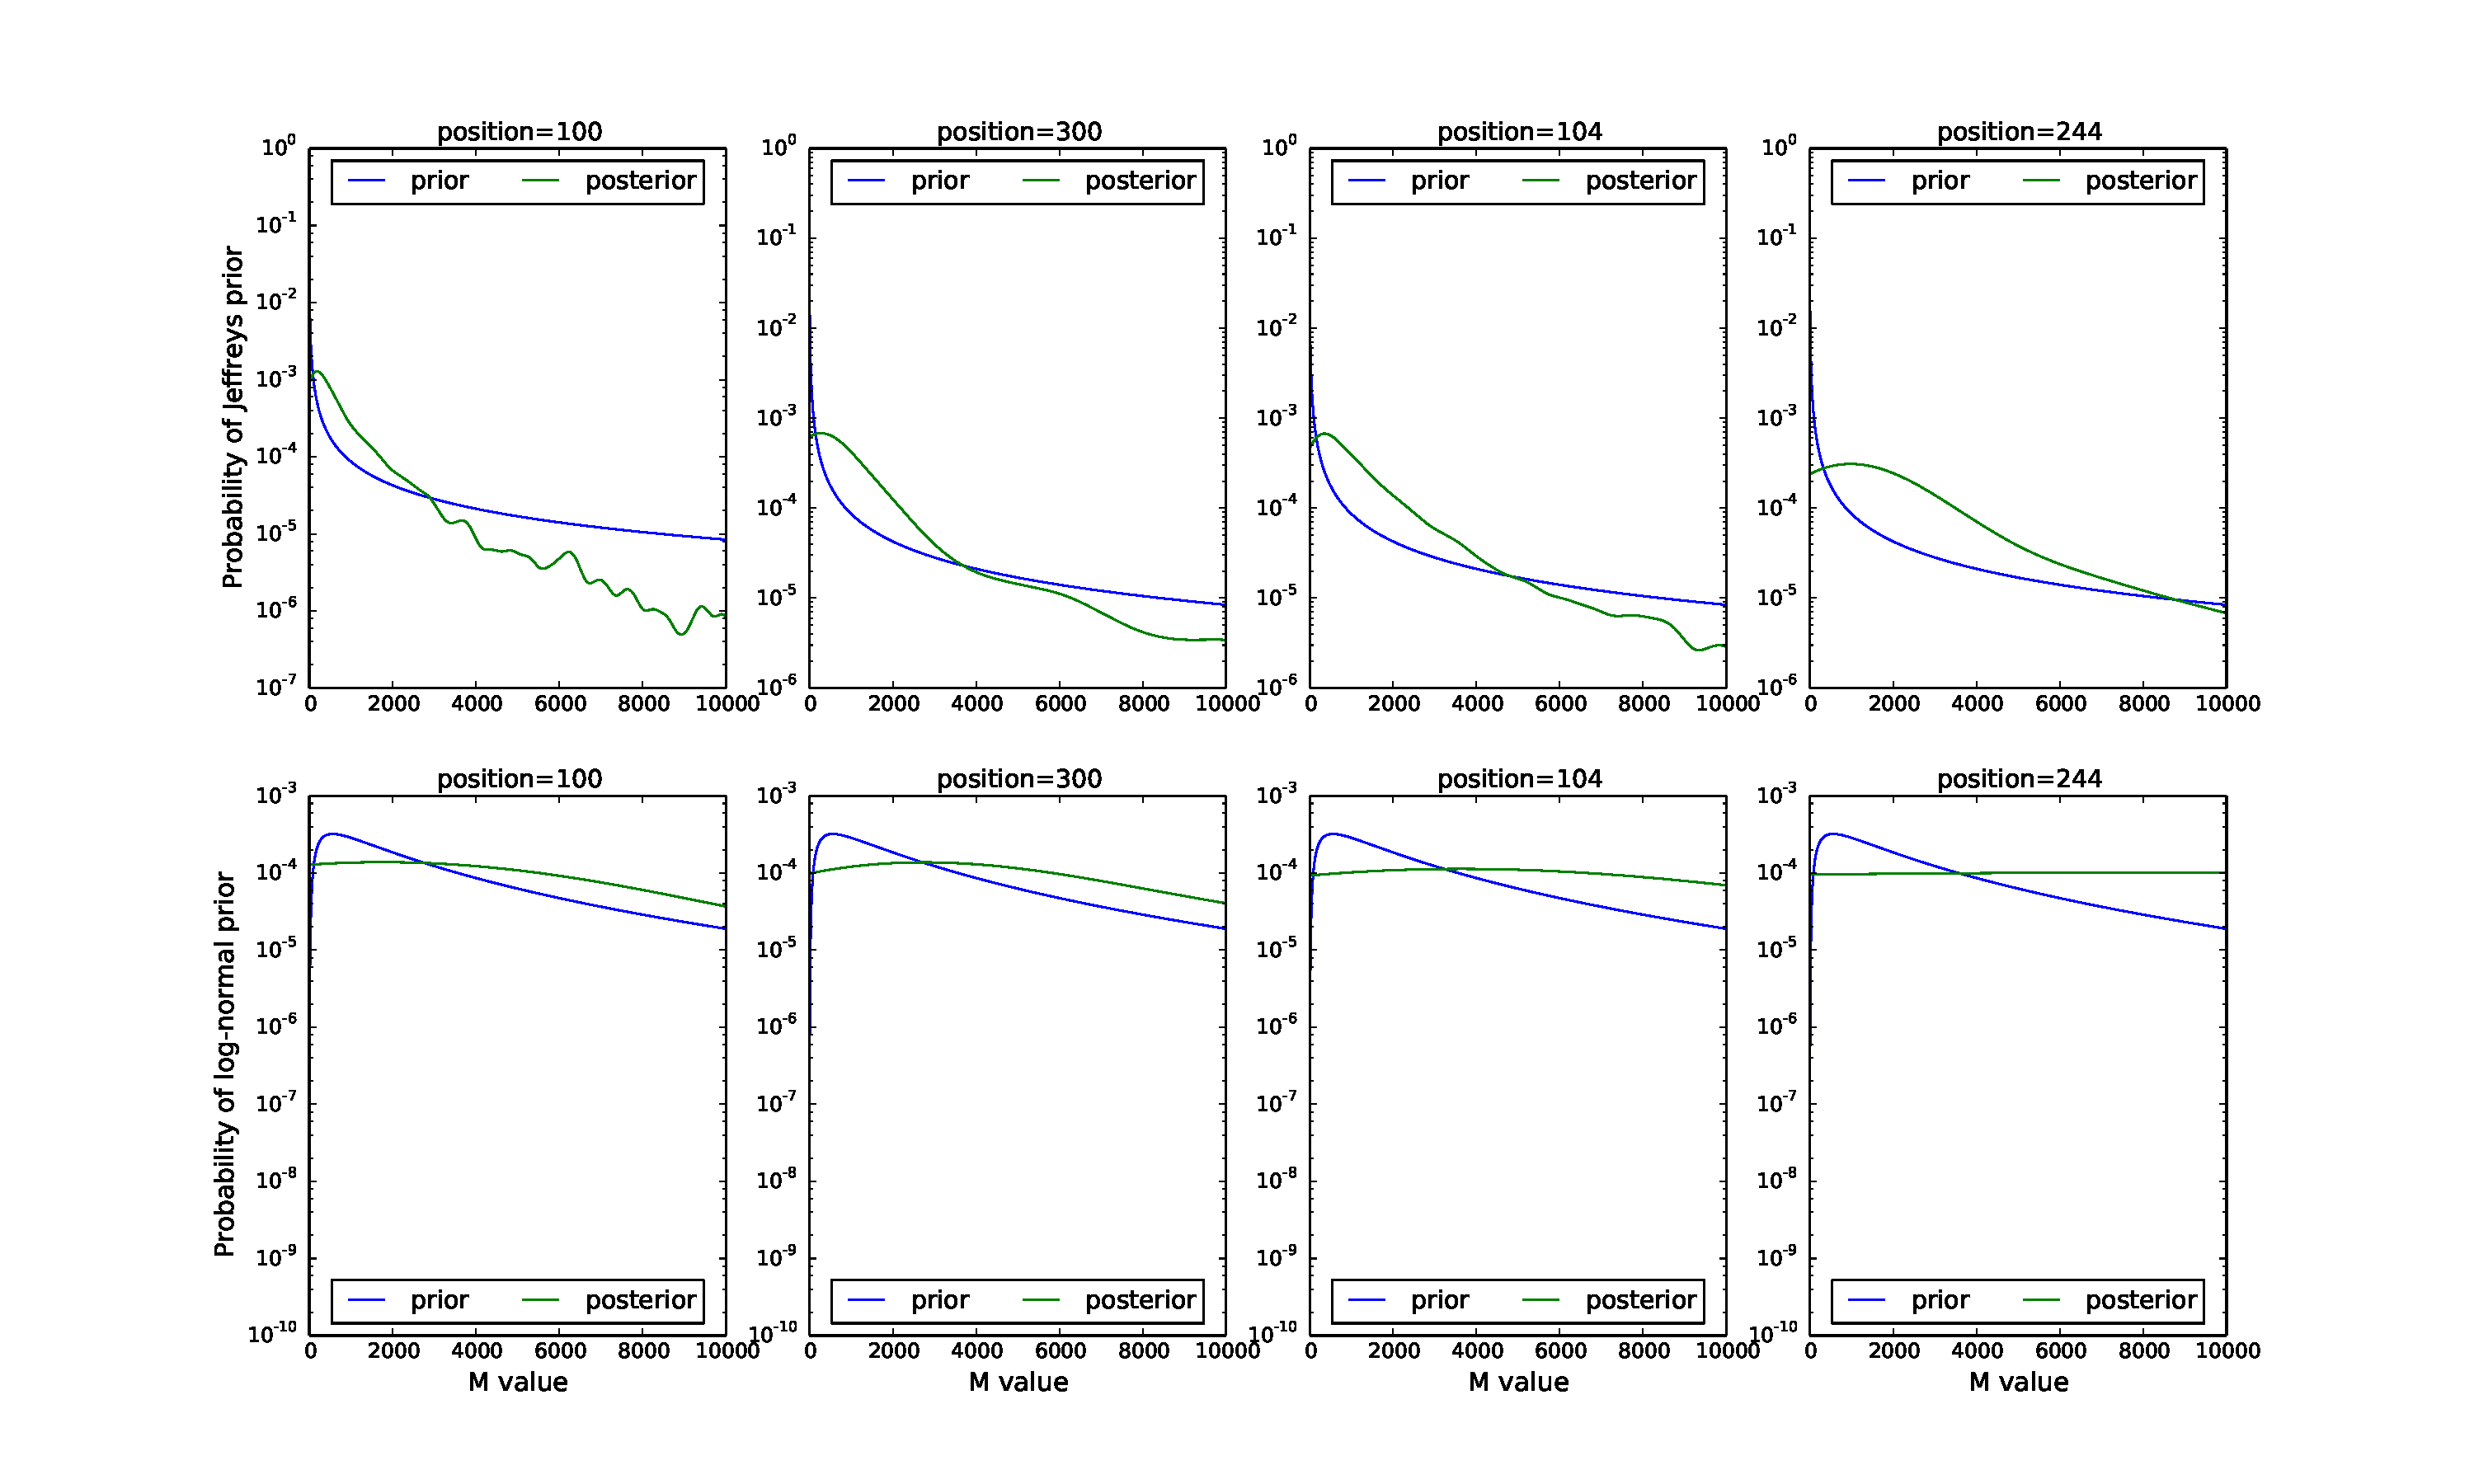
\includegraphics[width=170mm]{figs/post_prior_dilu_10.pdf}
\caption{Distribution of priors and posteriors when dilution is 10\%}
\label{fig:dilu_10}
\end{center}
\end{figure}

Statistically, We analyzed the posteriors and priors for Jeffreys prior and log-normal prior. Figure~\ref{fig:dilu_10} shows the probability distribution over different M values when dilution is 10\% at $100\times$ read depth rate. The positions are chosen in the middle of the base length- position 104 and 244 are mutant, and position 100 and 300 are non-mutant. From the posterior probability distributions are estimated by Gaussian Kernel Density [XXX]. From the figure non-mutant positions display normal and stable without a peak nor a strange shape. The Jeffreys' prior shows more information than the lognormal prior (flat) from the posterior curve. From the prior distribution, it shows our model wants to search for a small value for M.

%%%%%%%%%%%%%%%%%%%%%%%%%%%%%
% Results of priors on synthetic data
%%%%%%%%%%%%%%%%%%%%%%%%%%%%%
\subsection{Results of priors on synthetic data}
\subsubsection{Performance with read depth}

\begin{figure}[htbp]
\begin{center}
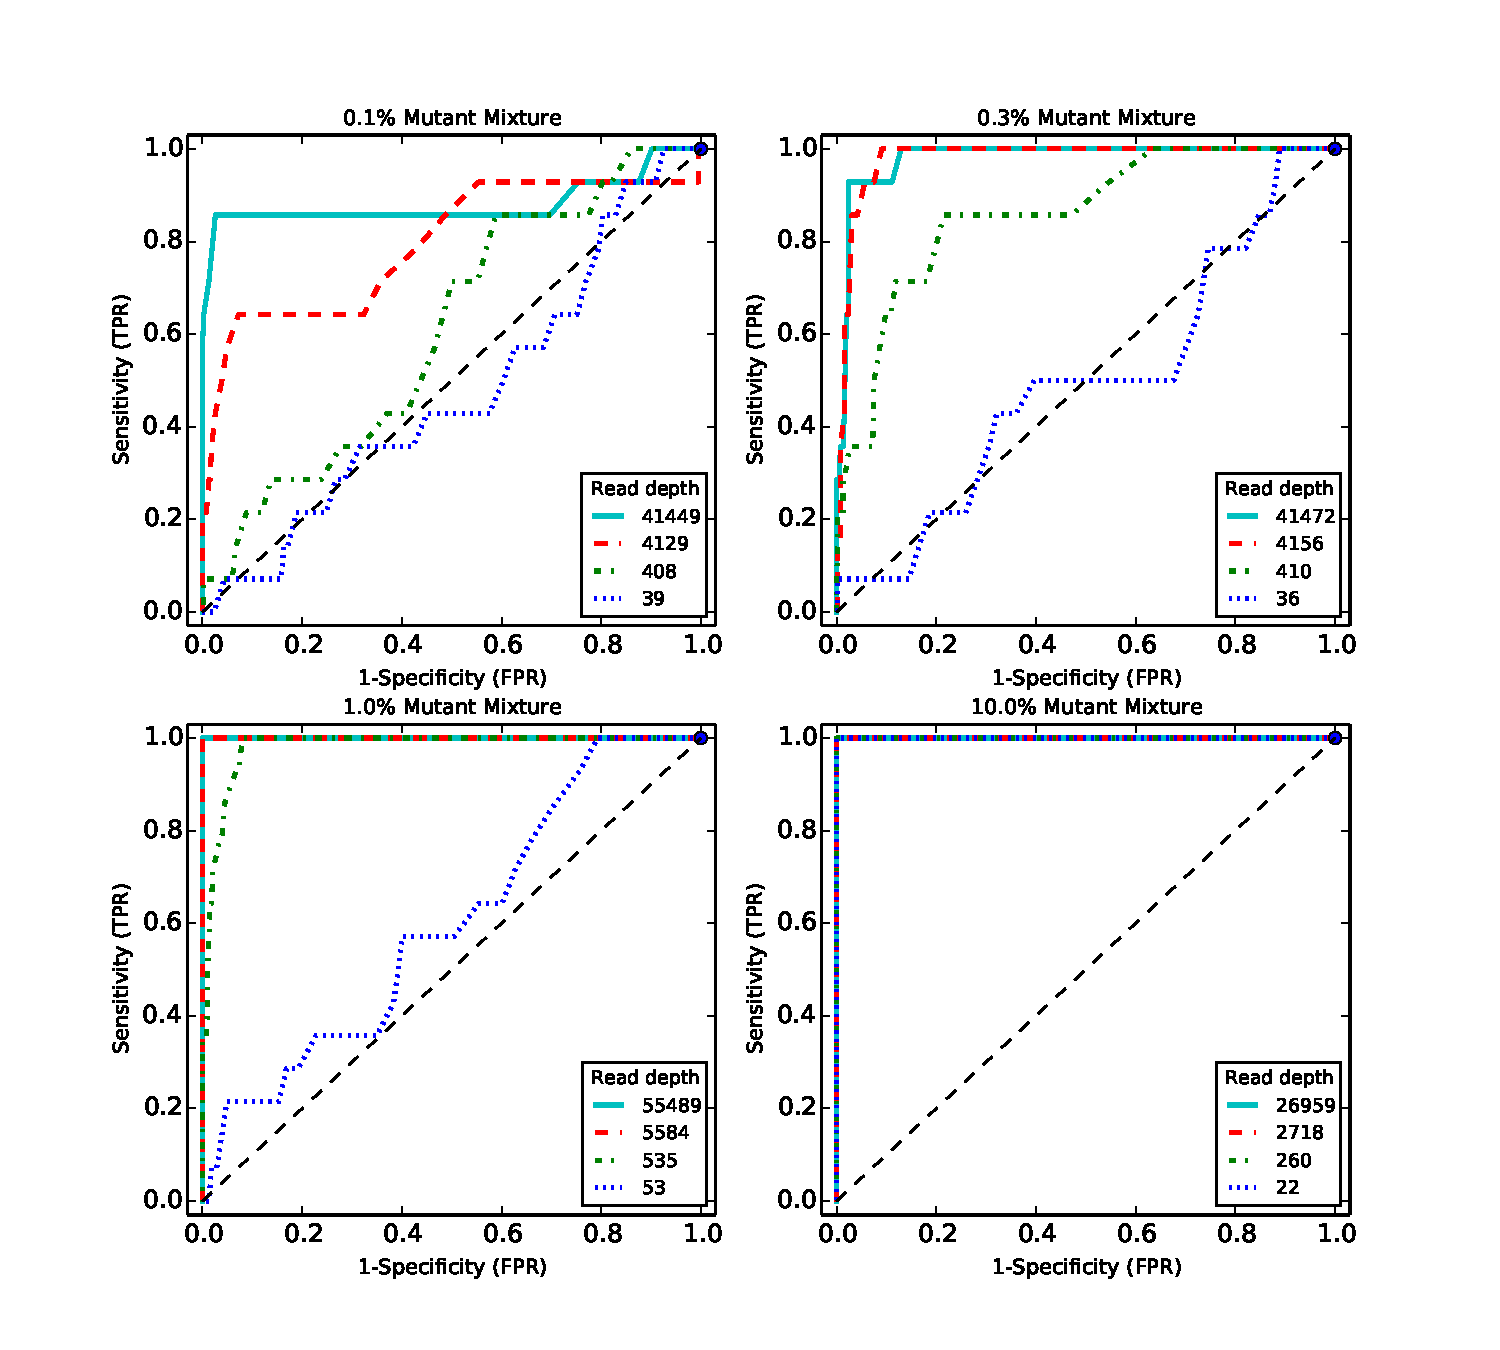
\includegraphics[width=120mm]{figs/ROC_without_chi2_jeffrey.pdf}
\caption{ROC curve for variants detection performance by Jeffreys prior.}
\label{fig:ROC_jeffrey}
\end{center}
\end{figure}

\begin{figure}[htbp]
\begin{center}
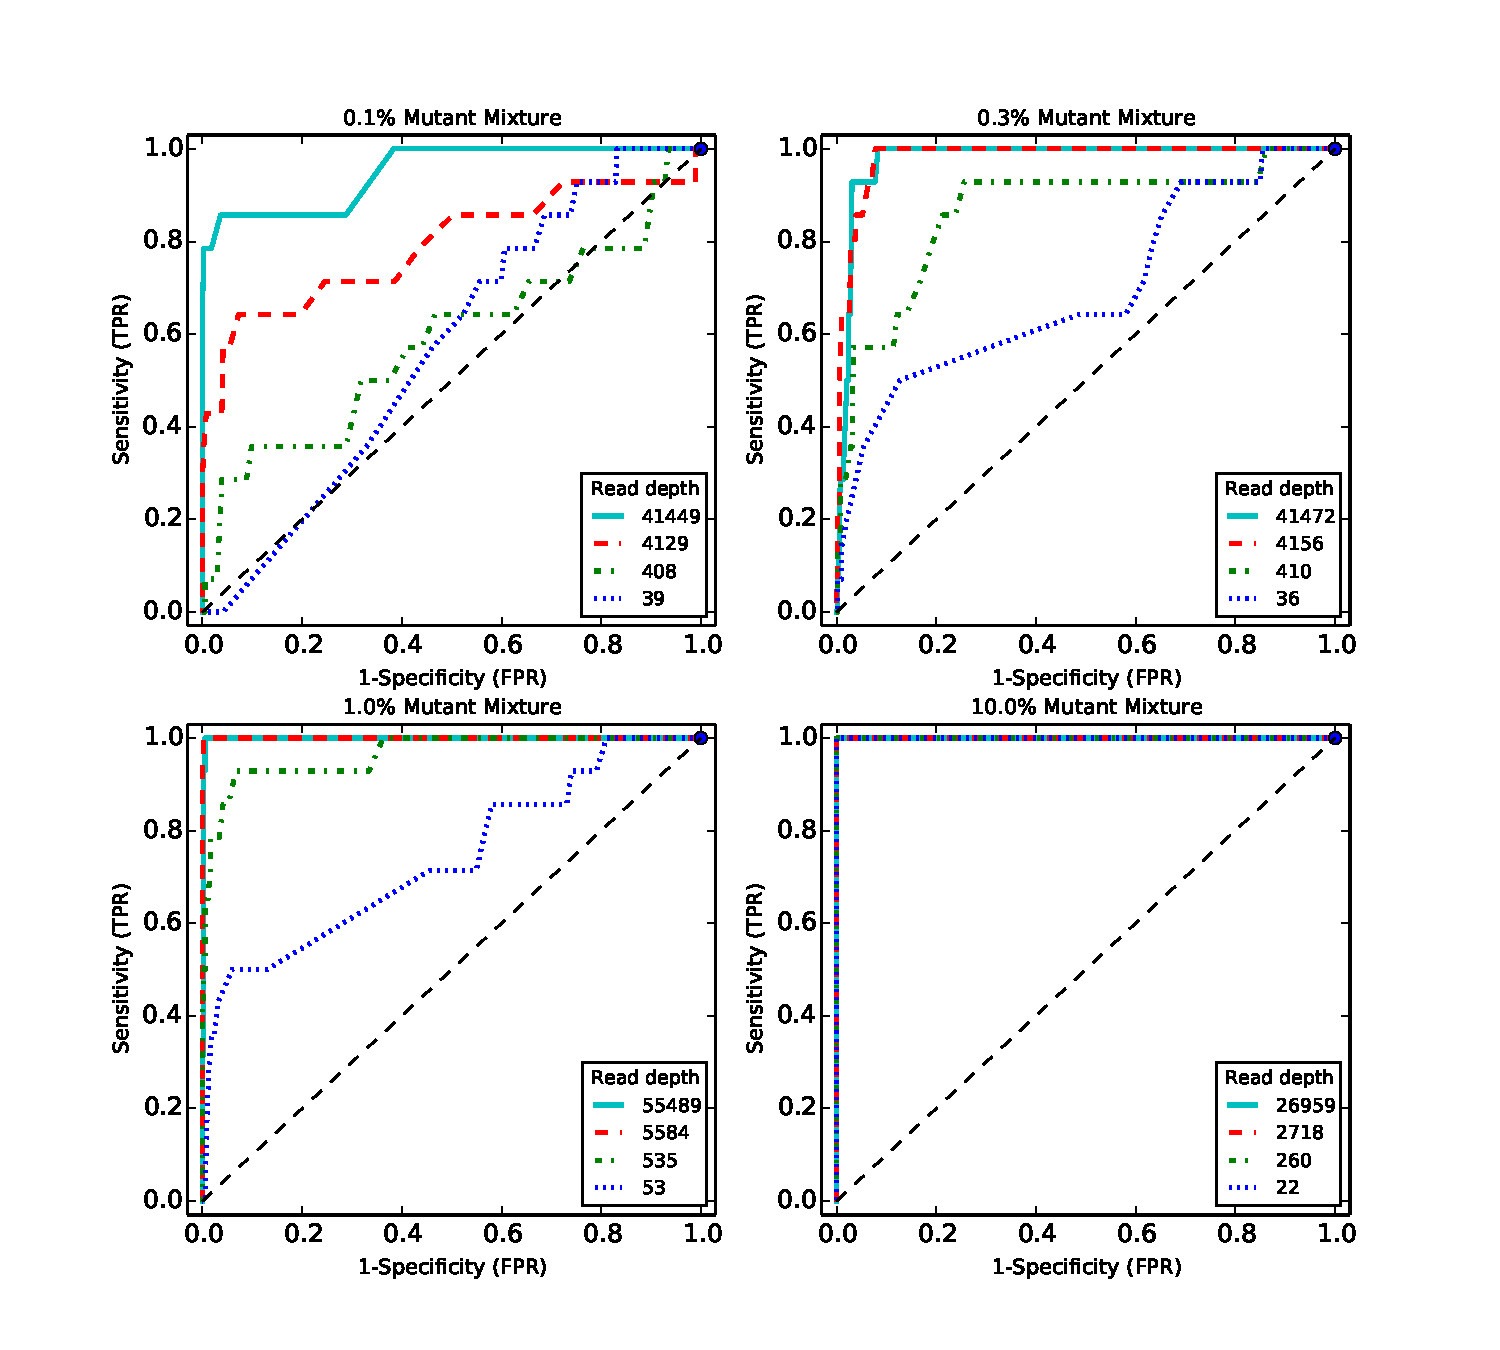
\includegraphics[width=120mm]{figs/ROC_without_chi2_lognormal.pdf}
\caption{ROC curve for variants detection performance by log-normal prior.}
\label{fig:ROC_lognormal}
\end{center}
\end{figure}


\begin{figure}[htbp]
\begin{center}
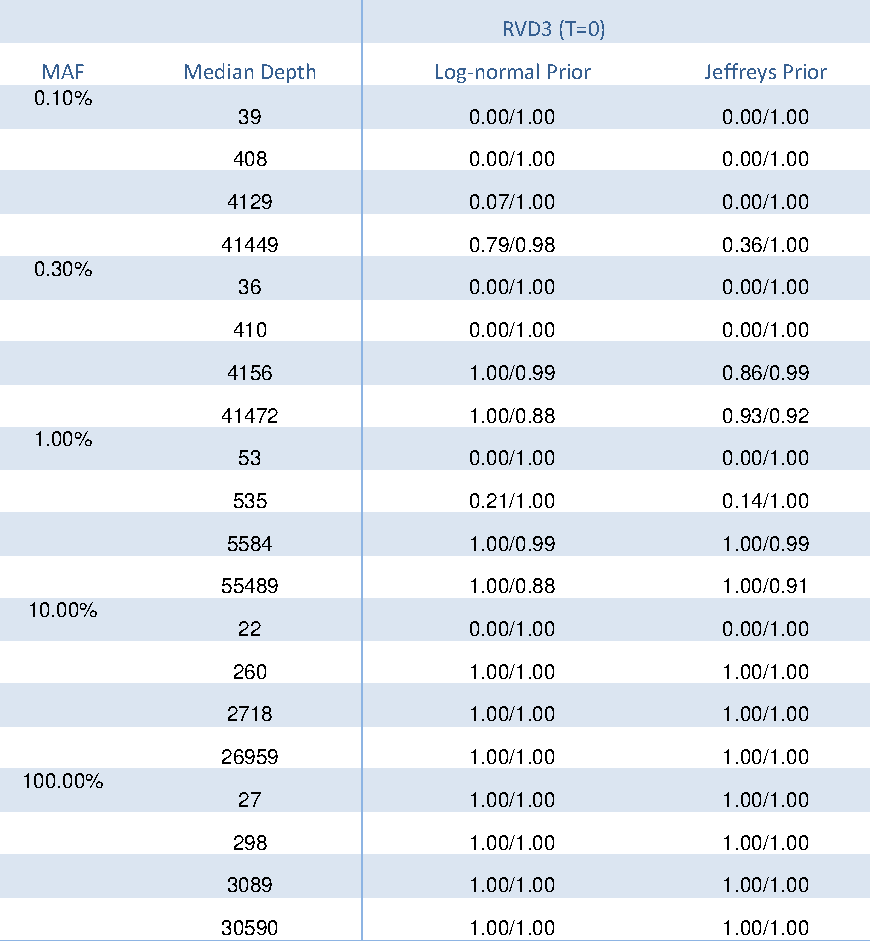
\includegraphics[width=160mm]{tables/Sen_Speci.pdf}
\caption{Sensitivity/Specificity comparison of RVD3 with different priors.}
\label{tbl:SS}
\end{center}
\end{figure}

\begin{figure}[htbp]
\begin{center}
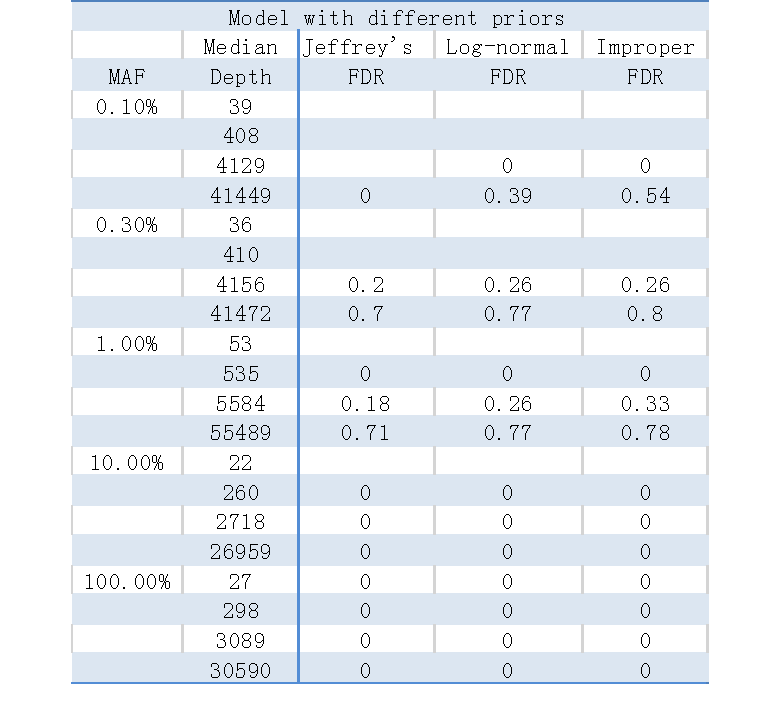
\includegraphics[width=160mm]{tables/FDR.pdf}
\caption{False Discovery Rate comparison of RVD3 with different priors.}
\label{tbl:FDR}
\end{center}
\end{figure}

To evaluate the performance of RVD3 model with priors, we generated receiver-operating characteristic curves (ROCs) for median read depth and minor allele frequencies (MAFs). Here the Bayesian test is used without the $\chi^2$ test. Figure~\ref{fig:ROC_jeffrey} and Figure~\ref{fig:ROC_lognormal} shows ROC curves with a fixed $\alpha=0.05$. The performance improves when the read depth goes up. (ROC shows that the model with priors performs better than improper prior situation especially on the small read depth). Noticed at the lowest depth (22) with 10.0\% mutant mixture, the sensitivity and specificity value are 1 and much better than the model with improper priors for $M_j$, which definitely demonstrates the advantage of priors.

\subsubsection{Sensitivity/Specificity/FDR}

Figure~\ref{tbl:SS} shows that the sensitivity and specificity of the RVD3 of different priors compared with the model with improper priors. Log-normal prior shows a higher sensitivity and specificity value than the Jeffreys prior.
Figure~\ref{tbl:FDR} shows the false discovery rate of the RVD3 with different priors. Jeffreys prior shows a smaller false discovery rate and higher accuracy than others. It is obvious no matter Jeffreys or log-normal, the variant detection performance acquires lower FDR than the model with improper priors. Based on the various advantages for Jeffreys and log-normal prior, RVD3 can afford a more appropriate choice for the precision parameter. Here we chose Jeffreys prior model because it's a non-information prior, and more attention should be paid to false discovery rate and accuracy for variants calling research, compared with the clinical experiment or diagnosis which cares more on true positive rate and true negative rate.
%%%%%%%%%%%%%%%%%%%%%%%%%%%%%%
% Results of Jeffreys prior on yeast data
%%%%%%%%%%%%%%%%%%%%%%%%%%%%%%
\subsection{Results of Jeffreys prior on yeast data}

We demonstrated our RVD3 model with Jeffreys prior on yeast data to identify the variants.


%%%%%%%%%%%%
% Discussion
%%%%%%%%%%%%
\section{Discussion}


\appendix

%%%%%%%%%%%%%%%%%%%
% Appendix A: Parameter Initialization
%%%%%%%%%%%%%%%%%%%
\section{Parameter Initialization}\label{sec:appendix_mom}
Since $r_{ji} \thicksim \text{Binomial}(n_{ji}, \theta_{ji})$, the first population moment is  $E[r_{ji}] = \theta_{ji} n_{ji}$ and the first sample moment is simply $m_1 = r_{ji}$. Therefore the MoM estimator is
\begin{equation}
	\tilde{\theta}_{ji} = \frac{r_{ji}} {n_{ji}}
\end{equation}

We take the MoM estimate, $\tilde{\theta}_{ji}$, as data for the next conditional distribution in the hierarchical model. The distribution is $\theta_{ji} \thicksim \text{Beta}(\mu_jM_j, (1-\mu_j)M_j)$. The first and second population moments are
\begin{eqnarray}
	E[\theta_{ji}] =& \mu_j,\\
	\text{Var}[\theta_{ji}] =& \frac{\mu_j(1-\mu_j)} { M_j + 1 }.
\end{eqnarray}
The first and second sample moments are $m_1 = \frac{1}{N}\sum_{i=1}^N \theta_{ji}$ and $m_2 = \frac{1}{N}\sum_{i=1}^N \theta_{ji}^2$. Setting the population moments equal to the sample moments and solving for $\mu_j$ and $M_j$ gives
\begin{eqnarray}
	\tilde{\mu}_j =& \frac{1}{N} \sum_{i=1}^N \theta_{ji}, \\
	\tilde{M_j} =& \frac{ \tilde{\mu}_j (1 - \tilde{\mu}_j ) } { \frac{1}{N} \sum_{i=1}^N \theta_{ji}^2 } -1.
\end{eqnarray}

Following the same procedure for the parameters of $\mu_j \thicksim \text{Beta}(\mu_0, M_0)$ gives the following MoM estimates
\begin{eqnarray}
	\tilde{\mu}_0 =& \frac{1}{J} \sum_{j=1}^J \mu_j \\
	\tilde{M}_0 =& \frac{ \tilde{\mu}_0 (1 - \tilde{\mu}_0 ) } {\frac{1}{J} \sum_{j=1}^J \mu_j^2 } -1.
\end{eqnarray}

%%%%%%%%%%%%%%%%%%%
% Appendix B: Inference of Jeffreys prior
%%%%%%%%%%%%%%%%%%%
\section{Inference of Jeffreys prior}\label{sec:appendix_mom}
We assume there is only one replicate,

\begin{equation}\label{eqn:Betapdf}
p\left({\theta }_{j} \right)= \frac{\Gamma \left({M}_{j} \right)}{\Gamma \left({\mu }_{j} {M}_{j}\right)\Gamma \left(( 1-{\mu }_{j}){M}_{j}\right)} {{\theta}_{j}}^{{\mu}_{j}{M}_{j}-1}{\left(1-\theta\right)_{j}}^{\left(1-{\mu}_{j}\right){M}_{j}-1}
\end{equation}

\begin{equation}\label{equ:JefferyInference1}
\begin{split}
\log p\left(\theta_{j}|\mu_{j},M_{j}\right)& =\log \Gamma \left(M_{j}\right)-\log \Gamma\left(\mu_{j},M_{j}\right)- \log \Gamma\left(1-\mu_{j},M_{j}\right)\\
& + (\mu_{j}M_{j}-1)\log\theta_{j} + ((1-\,u_{j})M_{j}-1)\log(1-\theta_{j})\
\end{split}
\end{equation}

\begin{equation}
\frac{\delta\log p(\theta_{j})}{\delta M_{j}} = \Psi(M_{j}) - \Psi(\mu_{j} M_{j})\mu_{j} - \Psi((1-\mu_{j})M_{j})(1-\mu_{j}) +\mu_{j}\log\theta_{j} + (1-\mu_{j})\log(1-\theta_{j})
\end{equation}

\begin{equation}
\frac{\delta^{2}\log p(\theta_{j})}{\delta M_{j}^{2}}  = \Psi_{1}(M_{j}) - \Psi_{1}(\mu_{j} M_{j})\mu_{j}^{2} - \Psi_{1}((1-\mu_{j})M_{j})(1-\mu_{j})^{2}
\end{equation}

Now we have the Jeffreys' prior for $M_{j}$:

\begin{equation}
[-\left(\Psi_{1}(M_{j}) - \Psi_{1}(\mu_{j} M_{j})\mu_{j}^{2} - \Psi_{1}((1-\mu_{j})M_{j}){(1-\mu_{j})^{2}}\right)]^{\frac{1}{2}}
\end{equation}

%%%%%%%%%%%%%%%%%%%
% Appendix C: Key parameters for RVD3 model with log-normal prior
%%%%%%%%%%%%%%%%%%%
\section{Key parameters for RVD3 model with log-normal prior}\label{sec:appendix_mom}
\begin{figure}[htbp]
\begin{center}
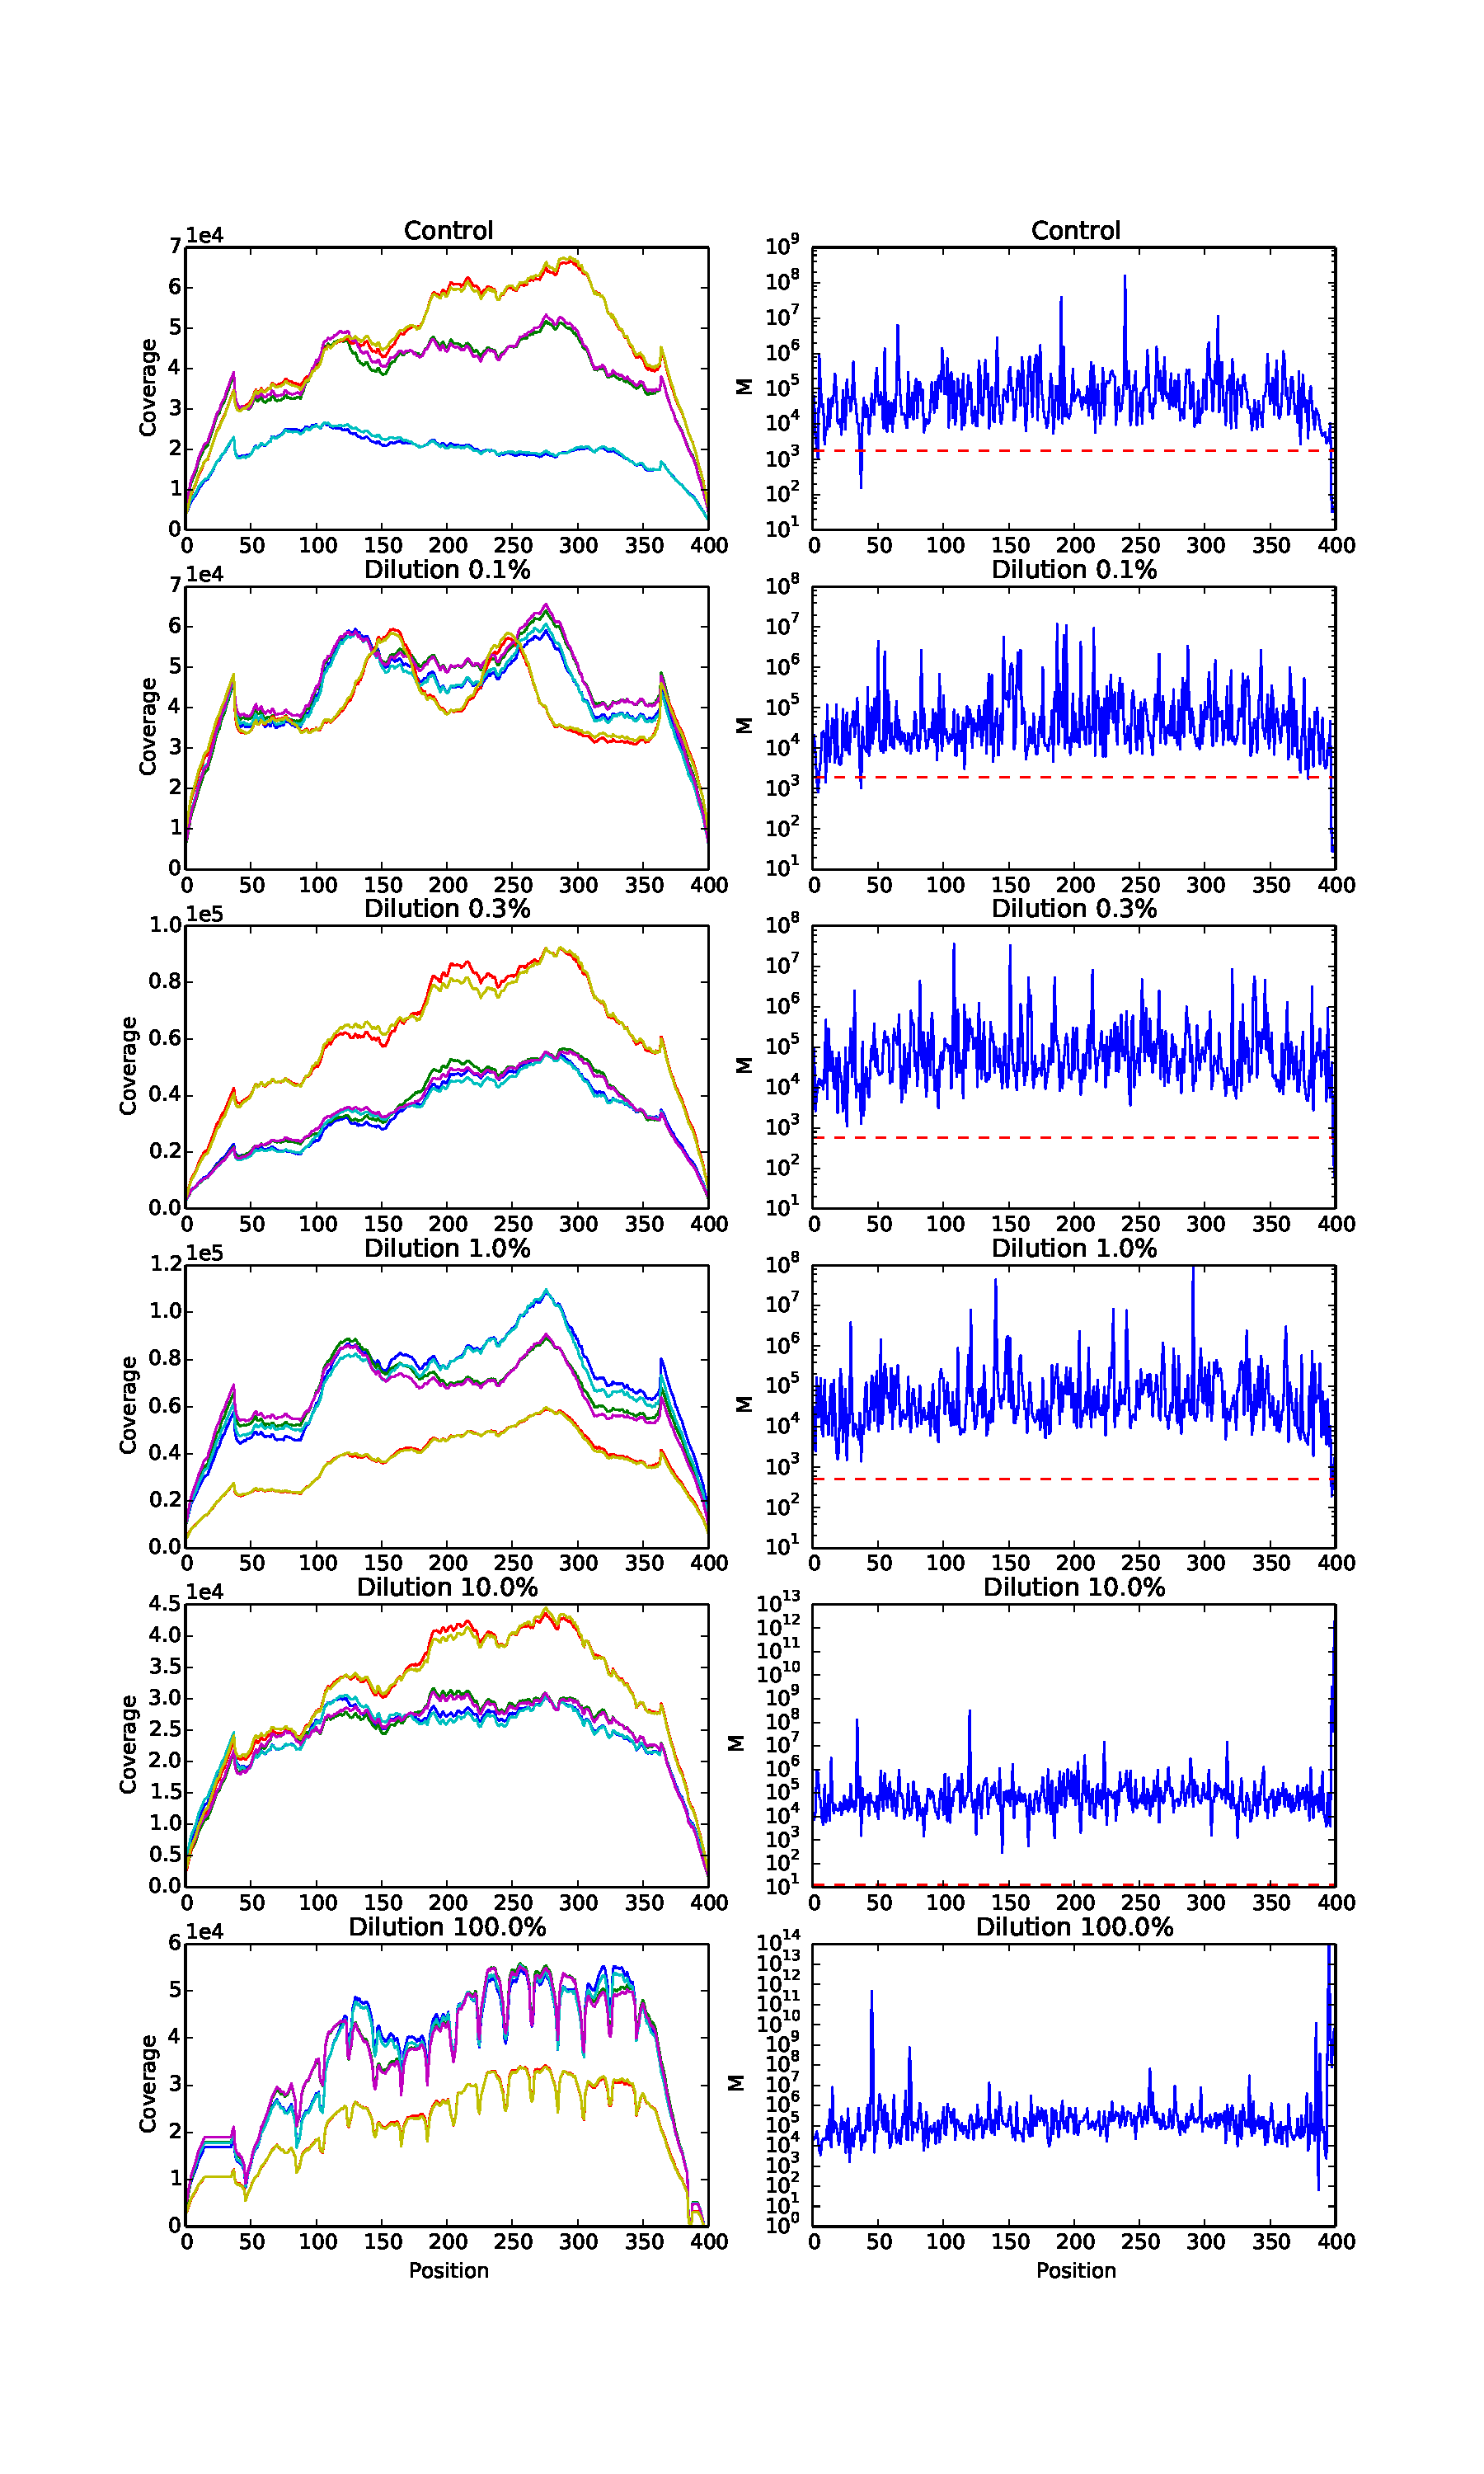
\includegraphics[width=120mm]{figs/M_lognormal.pdf}
\caption{Key parameters for RVD3 model with log-normal prior for synthetic DNA data sets.}
\label{fig:M_lognormal}
\end{center}
\end{figure}

\bibliographystyle{apalike}
\bibliography{bioinfo}
\end{document}
